%%%%%%%%%%%%%%%%%%%%%%%%%%%%%%%%%%%%%%%%%%%
%%% DOCUMENT PREAMBLE %%%
\documentclass[12pt]{report}
\usepackage[italian]{babel}

\usepackage[normalem]{ulem}
\useunder{\uline}{\ul}{}
\usepackage{longtable}
\usepackage{url}
\usepackage{placeins}
\usepackage[utf8x]{inputenc}
\usepackage{amsmath}
\usepackage{graphicx}
\graphicspath{{images/}}
\usepackage{parskip}
\usepackage{fancyhdr}
\usepackage{vmargin}
\usepackage{nameref}
\setmarginsrb{3 cm}{2.5 cm}{3 cm}{2.5 cm}{1 cm}{1.5 cm}{1 cm}{1.5 cm}

\title{uCOM}								
% Title
\author{Mazzaglia Pietro}						
% Author

\makeatletter
\let\thetitle\@title
\let\theauthor\@author
\newcommand*{\currentname}{\@currentlabelname}
\makeatother

\pagestyle{fancy}
\fancyhf{}
\lhead{\thetitle}
\rhead{\currentname}
\cfoot{\thepage}


\begin{document}
	
	\huge \textbf{Elaborazione - Iterazione 3}
	
	\renewcommand{\thesection}{\arabic{section}}
	
	\normalsize
	
	%%%%%%%%%%%%%%%%%%%%%%%% PIANIFICAZIONE %%%%%%%%%%%%%%%%%%%%%%

	\section{Introduzione}
	
	Nota la seguente tabella di pianificazione:
	
	
	% Please add the following required packages to your document preamble:
	% \usepackage{graphicx}
	\begin{table}[!htb]
		\centering
		\resizebox{\textwidth}{!}{%
			\begin{tabular}{|l|l|l|}
				\hline
				\textbf{Priorità} & \textbf{Requisiti  (Casi d'uso o funzionalità)}                                                                          & \textbf{Commento}                                                                                                                                                                                                                                \\ \hline
				\textbf{Alta}              & \begin{tabular}[c]{@{}l@{}}\textbf{Invia comunicazione}\\ \\ \textbf{Invia avviso}\\ \\ \textbf{Gestisce utente}\\ \\ \textbf{Effettua accesso}\end{tabular} & \begin{tabular}[c]{@{}l@{}}\textbf{Nucleo della piattaforma, alta frequenza}\\ \\ \textbf{Nucleo della piattaforma, alta frequenza}\\ \\ \textbf{Nucleo della piattaforma, sicurezza}\\ \\ \textbf{Nucleo della piattaforma, sicurezza, coinvolta in tutte le funzioni}\end{tabular} \\ \hline
				\textbf{Media}             & \begin{tabular}[c]{@{}l@{}}\textbf{Prenota pasto}\\ \\ \textbf{Richiede libro}\end{tabular}                                                & \begin{tabular}[c]{@{}l@{}}\textbf{Frequenza elevata e più parti interessate ma sostituibile}\\ \\ \textbf{Frequenza elevata e più parti interessate ma sostituibile}\end{tabular}                                                                                 \\ \hline
				Bassa             & \begin{tabular}[c]{@{}l@{}}Iscrive a un corso\\ \\ \textbf{Gestisce corso}\\ \\ Gestisce iscrizione corso\end{tabular}            & \begin{tabular}[c]{@{}l@{}}Bassa frequenza e sostituibile\\ \\ \textbf{Bassa frequenza e sostituibile}\\ \\ Bassa frequenza e sostituibile \end{tabular}                                                                                                                                                \\ \hline
			\end{tabular}%
		}
	\end{table}
	
	
	Gli obiettivi della terza iterazione sono:
	\begin{itemize}
		\item Analisi e progettazione, relativamente agli scenari dei casi d'uso \textit{UC1: Prenota Pasto}, \textit{UC2: Prenota libro} e \textit{UC5: Gestisce corso}.
		\item Miglioramenti al software risultante dall'Iterazione 2, secondo i criteri evidenziati durante l'Iterazione 2
		\item Implementazione di \textit{UC5} e di uno scenario d'uso di successo tra \textit{UC1} e \textit{UC2} 
		\item Tentativo di integrazione di parti di interfaccia grafica per testare la flessibilità del software
	\end{itemize}
	
	Alcune tra i requisiti più critici dell'applicazione sono già state trattati, tra cui Affidabilità, Sicurezza, Automatizzazione, dunque maggiore attenzione verrà posta in questa iterazione sull'Integrazione con altri sistemi e sul requisito di Flessibilità di \textit{uCOM}.
	
	\newpage
	
	\section{Modello dei casi d'uso}
	
	Seguono descrizioni dettagliate dei casi d'uso \textit{UC1}, \textit{UC2} e \textit{UC5}.
	
	Inoltre si presentano i \textit{Diagrammi di sequenza di sistema} relativi agli scenari di successo e i \textit{Contratti delle operazioni}.
	
	\subsection{UC1: Prenota pasto}

	% Please add the following required packages to your document preamble:
% \usepackage{longtable}
% Note: It may be necessary to compile the document several times to get a multi-page table to line up properly
\begin{longtable}{|l|l|}
	\hline
	\textbf{Nome caso d'uso} & UC1: Prenota pasto \\ \hline
	\endfirsthead
	%
	\endhead
	%
	\textbf{Portata} & Piattaforma uCOM \\ \hline
	\textbf{Livello} & Obiettivo utente \\ \hline
	\textbf{Attore primario} & Studente \\ \hline
	\textbf{\begin{tabular}[c]{@{}l@{}}Parti interessate \\ e Interessi\end{tabular}} & \begin{tabular}[c]{@{}l@{}}Studente: vuole prenotare pasto alla mensa per il giorno\\ successivo.\\ \\ Servizio Mensa: vuole ricevere la prenotazione\\ dello studente, che deve essere coerente con il menù offerto.\\ \\ Direzione Campus: vuole che i propri studenti possano\\ interagire con Servizi Esterni affiliati al Campus, come la mensa\end{tabular} \\ \hline
	\textbf{Pre-condizioni} & Lo Studente possiede un account sulla piattaforma. \\ \hline
	\textbf{Garanzia di successo} & Lo Studente ha ricevuto conferma dell'operazione. \\ \hline
	\textbf{\begin{tabular}[c]{@{}l@{}}Scenario principale \\ di successo\end{tabular}} & \begin{tabular}[c]{@{}l@{}}1. Lo Studente effettua l'accesso\\ 2. Lo Studente avvia l'operazione di prenotazione pasto.\\ 3. Lo Studente indica per quale pasto vuole prenotare\\ 4. Il Sistema mostra il menù relativo a tale pasto\\ 5. Lo Studente inserisce le proprie scelte.\\ 6. Lo Studente invia la prenotazione del pasto.\\ 7. Il Sistema elabora la prenotazione.\\ 8. Il Sistema conferma la riuscita dell'operazione.\end{tabular} \\ \hline
	\textbf{Estensioni} & \begin{tabular}[c]{@{}l@{}}*a. In qualsiasi momento.Il Sistema non è in grado di funzionare\\ correttamente in un dato momento.\\ \\  \quad   1) Il Sistema segnala l'impossibilità di eseguire l'azione.\\ \\  \quad   - Lo Studente riprova a eseguire l'azione dopo un certo periodo\\     di tempo.\end{tabular} \\ \hline
	\textbf{Estensioni} & \begin{tabular}[c]{@{}l@{}}*b. In qualsiasi momento. Il Sistema entra in uno stato di errore\\ irrisolvibile.\\ \\   \quad  1) Il Sistema termina la sessione, perdendo i dati.\\ \\     \quad- Lo Studente deve ricominciare l'operazione.\\ \\ *c. In qualsiasi momento. Lo Studente interrompe l'operazione.\\ \\ \quad 1) Il Sistema termina l'operazione.\\ \\ 3a. Lo Studente indica un'opzione non valida o possibile.\\ \\     \quad1) Il Sistema richiede nuova immissione dei dati allo Studente.\\ \\ 5a. Lo Studente inserisce informazioni non valide.\\ \\     \quad1) Il Sistema richiede nuova immissione dei dati allo Studente\\ \\ 7a. Il Sistema invia la prenotazione a un Servizio Esterno.\\ \\   \quad  1a) Il Servizio Esterno riceve correttamente la prenotazione.\\  \\         \quad\quad2) Il Sistema conferma la riuscita dell'operazione.\\ \\     \quad1b) Il Servizio Esterno rigetta la richiesta.\\ \\         \quad\quad2a) Il Sistema va in errore temporaneo.\\ \\         \quad\quad- Lo Studente può ritentare l'operazione dopo un certo\\           periodo di tempo.\\ \\         \quad\quad2b) Una regola di domio è stata violata, dunque viene\\         restituito un messaggio di errore.\\ \\          \quad\quad- Potrebbe essere richiesto l'inserimento di nuovi dati.         \\ \\ 7b. Il Sistema gestisce internamente la prenotazione.\end{tabular} \\ \hline
	\textbf{Requisiti speciali} & \begin{tabular}[c]{@{}l@{}}- Lo Studente deve inserire dati che siano conformi al menù \\ offerto dal Servizio Mensa\end{tabular} \\ \hline
	\textbf{\begin{tabular}[c]{@{}l@{}}Elenco delle varianti \\ tecnologiche e dei dati\end{tabular}} & \begin{tabular}[c]{@{}l@{}}3/5) L'inserimento delle informazioni può avvenire attraverso\\ metodi input diversi, come tastiera e mouse o un touchscreen.\\ \\ 7) La richiesta potrebbe venire rigettata dal servizio interno o \\ esterno in quanto una prenotazione è gia disponibile. In tal caso\\ si potrebbe proporre l'aggiornamento della \\prenotazione all'utente.\\ \\ 7b) L'elaborazione di sistema può avvenire internamente tramite\\ un Registro Prenotazioni relativo al giorno successivo, che viene\\ inoltrato quotidianamente al Servizio Mensa.\end{tabular} \\ \hline
	\textbf{Frequenza di ripetizione} & giornaliera \\ \hline
	\textbf{Varie} & \begin{tabular}[c]{@{}l@{}}Si potrebbe prevedere un sistema che permetta l'inserimento\\ offline e l'elaborazione non appena il servizio ritorna disponibile.\\ \\ La prenotazione viene registrata dal Sistema se viene elaborata\\ esternamente?\\ \\ Si possono prevedere meccanismi di recupero dell'istanza in\\ caso di errori gravi.\end{tabular} \\ \hline
\end{longtable}	

	\newpage

	\subsection{UC2: Richiede libro}

	% Please add the following required packages to your document preamble:
% \usepackage{longtable}
% Note: It may be necessary to compile the document several times to get a multi-page table to line up properly
\begin{longtable}{|l|l|}
	\hline
	\textbf{Nome caso d'uso} & UC2: Richiede libro \\ \hline
	\endfirsthead
	%
	\endhead
	%
	\textbf{Portata} & Piattaforma uCOM \\ \hline
	\textbf{Livello} & Obiettivo utente \\ \hline
	\textbf{Attore primario} & Studente \\ \hline
	\textbf{\begin{tabular}[c]{@{}l@{}}Parti interessate \\ e Interessi\end{tabular}} & \begin{tabular}[c]{@{}l@{}}Studente: vuole richiedere un libro alla biblioteca\\ del Campus.\\ \\ Biblioteca: vuole ricevere la richiesta del libro da parte\\ dello studente, in conformità con la disponibilità dei libri\\ \\ Direzione Campus: vuole che i propri studenti possano\\ interagire con Servizi affiliati al Campus, come la biblioteca\end{tabular} \\ \hline
	\textbf{Pre-condizioni} & Lo Studente possiede un account sulla piattaforma. \\ \hline
	\textbf{Garanzia di successo} & Lo Studente ha ricevuto conferma dell'operazione. \\ \hline
	\textbf{\begin{tabular}[c]{@{}l@{}}Scenario principale \\ di successo\end{tabular}} & \begin{tabular}[c]{@{}l@{}}1. Lo Studente effettua l'accesso\\ 2. Lo Studente avvia l'operazione di richiesta libro.\\ 3. Il Sistema mostra i libri disponibili\\ 4. Lo Studente inserisce il libro e la durata \\ prevista per la richiesta.\\ 5. Lo Studente invia la richiesta libro.\\ 6. Il Sistema elabora la richiesta.\\ 7. Il Sistema conferma la riuscita dell'operazione.\end{tabular} \\ \hline
	\textbf{Estensioni} & \begin{tabular}[c]{@{}l@{}}*a. In qualsiasi momento.Il Sistema non è in grado di funzionare \\ correttamente in un dato momento.\\ \\  \quad   1) Il Sistema segnala l'impossibilità di eseguire l'azione.\\ \\   \quad  - Lo Studente riprova a eseguire l'azione dopo un certo periodo\\     di tempo.\end{tabular} \\ \hline
	\textbf{Estensioni} & \begin{tabular}[c]{@{}l@{}}*b. In qualsiasi momento. Il Sistema entra in uno stato di errore\\ irrisolvibile.\\ \\   \quad  1) Il Sistema termina la sessione, perdendo i dati.\\ \\     \quad- Lo Studente deve ricominciare l'operazione.\\ \\ *c. In qualsiasi momento. Lo Studente interrompe l'operazione.\\ \\ \quad1) Il Sistema termina l'operazione.\\ \\ 4a. Lo Studente inserisce dati non validi.\\ \\     \quad1) Il Sistema richiede nuova immissione dei dati allo Studente.\\ \\ 6a. Il Sistema invia la richiesta a un Servizio Esterno.\\ \\     \quad1a) Il Servizio Esterno riceve correttamente la richiesta.\\  \\         \quad\quad2) Il Sistema conferma la riuscita dell'operazione.\\ \\     \quad1b) Il Servizio Esterno rigetta la richiesta.\\ \\         \quad\quad2a) Il Sistema va in errore temporaneo.\\ \\         \quad- Lo Studente può ritentare l'operazione dopo un certo\\           periodo di tempo.\\ \\         \quad\quad2b) Una regola di dominio è stata violata, dunque viene\\         restituito un messaggio di errore.\\ \\          \quad\quad- Potrebbe essere richiesto l'inserimento di nuovi dati.         \\ \\ 6b. Il Sistema gestisce internamente la richiesta.\end{tabular} \\ \hline
	\textbf{Requisiti speciali} & \begin{tabular}[c]{@{}l@{}}- Lo Studente deve inserire dati che siano conformi ai libri\\ disponibili in Biblioteca\end{tabular} \\ \hline
	\textbf{\begin{tabular}[c]{@{}l@{}}Elenco delle varianti \\ tecnologiche e dei dati\end{tabular}} & \begin{tabular}[c]{@{}l@{}}4) L'inserimento delle informazioni può avvenire attraverso\\ metodi input diversi, come tastiera e mouse o un touchscreen.\\ \\ 7b) L'elaborazione di sistema può avvenire internamente se il\\ servizio di gestione della biblioteca viene integrato in uCOM.\end{tabular} \\ \hline
	\textbf{Frequenza di ripetizione} & media-alta \\ \hline
	\textbf{Varie} & \begin{tabular}[c]{@{}l@{}}Si potrebbe prevedere un sistema che permetta l'inserimento\\ offline e l'elaborazione non appena il servizio ritorna disponibile.\\ \\ La richiesta viene registrata dal Sistema se viene elaborata\\ esternamente?\\ \\ Si possono prevedere meccanismi di recupero dell'istanza in\\ caso di errori gravi.\end{tabular} \\ \hline
\end{longtable}	

	\newpage

	\subsection{UC5: Gestisce corso}

	Questo caso d'uso è di tipo CRUD (Create Read Update Delete). Ai fini dello sviluppo di una versione di prova di \textit{uCOM} sarà trattato solo uno dei quattro scenari, ovvero quello di Creazione del corso. Gli altri scenari saranno considerati come estensioni del caso d'uso.

	% Please add the following required packages to your document preamble:
% \usepackage[normalem]{ulem}
% \useunder{\uline}{\ul}{}
% \usepackage{longtable}
% Note: It may be necessary to compile the document several times to get a multi-page table to line up properly
\begin{longtable}{|l|l|}
	\hline
	\textbf{Nome caso d'uso} & UC5: Gestisce corso \\ \hline
	\endfirsthead
	%
	\endhead
	%
	\textbf{Portata} & Piattaforma uCOM \\ \hline
	\textbf{Livello} & Obiettivo utente (CRUD) \\ \hline
	\textbf{Attore primario} & Amministratore \\ \hline
	\textbf{\begin{tabular}[c]{@{}l@{}}Parti interessate \\ e Interessi\end{tabular}} & \begin{tabular}[c]{@{}l@{}}Amministratore: vuole poter gestire la creazione di un corso\\ svolto internamente al Campus\\ \\ Direzione Campus: vuole che la gestione dei corsi che si\\ svolgono all'interno del Campus siano gestite internamente dal\\ personale del Campus (Amministrazione)\end{tabular} \\ \hline
	\textbf{Pre-condizioni} & L'Amministratore possiede un account sulla piattaforma \\ \hline
	\textbf{Garanzia di successo} & \begin{tabular}[c]{@{}l@{}}Un nuovo corso è stato creato.\\ L'Amministratore ha ricevuto conferma dell'operazione.\end{tabular} \\ \hline
	\textbf{\begin{tabular}[c]{@{}l@{}}Scenario principale \\ di successo\end{tabular}} & \begin{tabular}[c]{@{}l@{}}1. L'Amministratore effettua l'accesso.\\ 2. L'Amministratore avvia la creazione di un corso.\\ 3. L'Amministratore inserisce nome e descrizione del corso.\\ 4. L'Amministratore aggiunge il corso al Sistema.\\ 5. Il Sistema aggiunge il corso al proprio Registro Corsi.\\ 6. Il Sistema conferma la riuscita dell'operazione.\end{tabular} \\ \hline
	\textbf{Estensioni} & \begin{tabular}[c]{@{}l@{}}*a. In qualsiasi momento.Il Sistema non è in grado di funzionare\\ correttamente in un dato momento.\\ \\ \quad1) Il Sistema segnala l’impossibilità a di eseguire l’azione. \\ \\ \quad- L'Amministratore riprova a eseguire l’azione dopo un certo \\ periodo di tempo.\\ \\ *b. In qualsiasi momento. Il Sistema entra in uno stato di errore \\ irrisolvibile. \\ \\ \quad1) Il Sistema termina la sessione, perdendo i dati. \\ \\ \quad- L'Amministratore deve ricominciare l’operazione.\\ \\ *c. In qualsiasi momento. L'Amministratore interrompe \\ l’operazione. \\ \\ \quad1) Il Sistema termina l’operazione.\\ \\ 2a. L'Amministratore avvia la lettura dei dati di un corso.\\ \\ \quad1) L'Amministratore inserisce il nome del Corso.\\ \\ \quad2) L'Amministratore richiede la lettura dei dati del corso.\\ \\ \quad3) Il Sistema preleva i dati del corso richiesto \\ dal Registro Corsi.\\ \\ \quad4) Il Sistema restituisce i dati del corso richiesto.\end{tabular} \\ \hline
	\textbf{Estensioni} & \begin{tabular}[c]{@{}l@{}}2b. L'Amministratore avvia la modifica di un corso.\\ \\ \quad1) L'Amministratore inserisce le informazioni del corso\\ da modificare.\\ \\ \quad2) L'Amministratore modifica il corso.\\ \\ \quad3) Il Sistema aggiorna il corso sul Registro Corsi.\\ \\ \quad4) Il Sistema conferma la riuscita dell'operazione.\\ \\ 2c. L'Amministratore avvia l'eliminazione di un corso.\\ \\ \quad1) L'Amministratore inserisce le informazioni del corso\\ da eliminare.\\ \\ \quad2) L'Amministratore elimina il corso.\\ \\ \quad3) Il Sistema elimina il corso dal Registro Corsi.\\ \\ \quad4) Il Sistema conferma la riuscita dell'operazione.\\ \\ 3a. L'Amministratore inserisce informazioni non valide. \\ \\ \quad1) Il Sistema richiede nuova immissione dei dati \\ all'Amministratore\end{tabular} \\ \hline
	\textbf{Requisiti speciali} & Nessuno \\ \hline
	\textbf{\begin{tabular}[c]{@{}l@{}}Elenco delle varianti \\ tecnologiche e dei dati\end{tabular}} & \begin{tabular}[c]{@{}l@{}}3) L'inserimento delle informazioni può avvenire attraverso\\ metodi input diversi, come tastiera e mouse o un touchscreen.\end{tabular} \\ \hline
	\textbf{Frequenza di ripetizione} & frequenza medio-bassa \\ \hline
	\textbf{Varie} & \begin{tabular}[c]{@{}l@{}}Si potrebbero aggiungere nuove informazioni da memorizzare sul\\ Registro Corsi.\end{tabular} \\ \hline
\end{longtable}	
	
	\newpage
	
	%%%%%%%%%%%%%% ANALISI ORIENTATA AGLI OGGETTI %%%%%%%%%%%%%%%%%
	
	\section{Modello di dominio}
	
	\subsection{Introduzione}
	
	Sulla base dei casi d'uso finora analizzati sono state identificate le seguenti classi concettuali:
	\begin{itemize}
		\item \textbf{Pasto}
		\item \textbf{Prenotazione Pasto}		
		\item \textbf{Libro}
		\item \textbf{Richiesta Libro}
		\item \textbf{Corso}
		\item \textbf{Registro Corsi}
	\end{itemize}

	Tenendo conto di associazioni e attributi, a partire dallo schema dell'Iterazione 1, è stato ricavato il seguente Modello di Dominio:
	
	\begin{center}	
	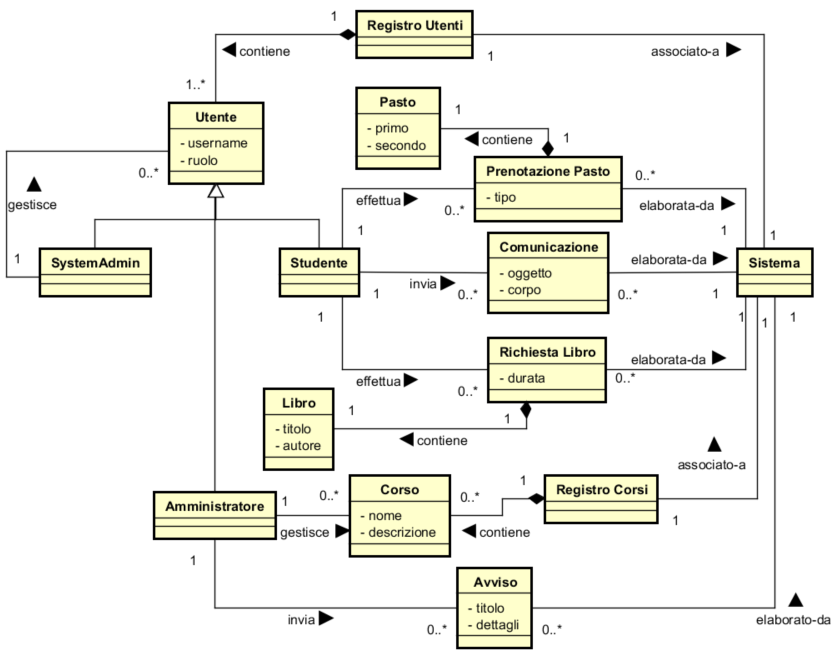
\includegraphics[scale=0.75]{./images/domain-I3.png}
	\end{center}
	
	I dettagli relativi alle classi sono stati inseriti nel \textbf{Glossario}.
	
	\newpage
	
	\section{Diagrammi di sequenza di sistema e contratti delle operazioni}
	
	I diagramma di sequenza di sistema mostrano gli eventi di I/O del sistema \textit{uCOM}, descrivendo in maniera chiara le interazioni tra attori e sistema.
	
	\subsection{UC1: Prenota pasto}
	\begin{center}
		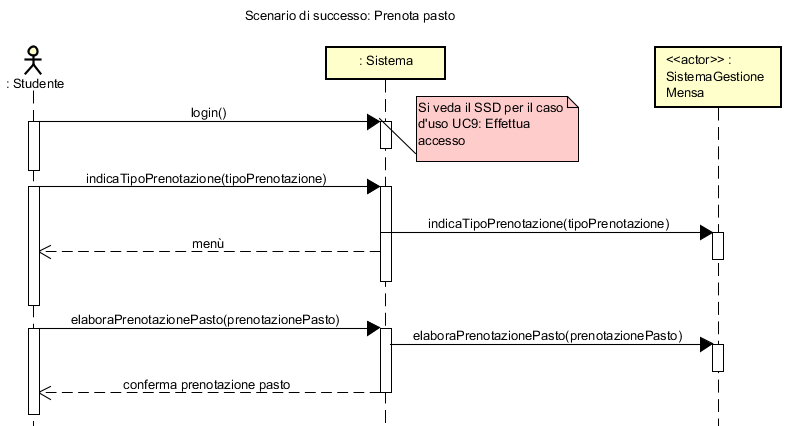
\includegraphics{./images/SSD_UC1.png}
	\end{center}
	
	\newpage	
		
	\subsection{UC2: Richiede libro}
	
	\begin{center}
		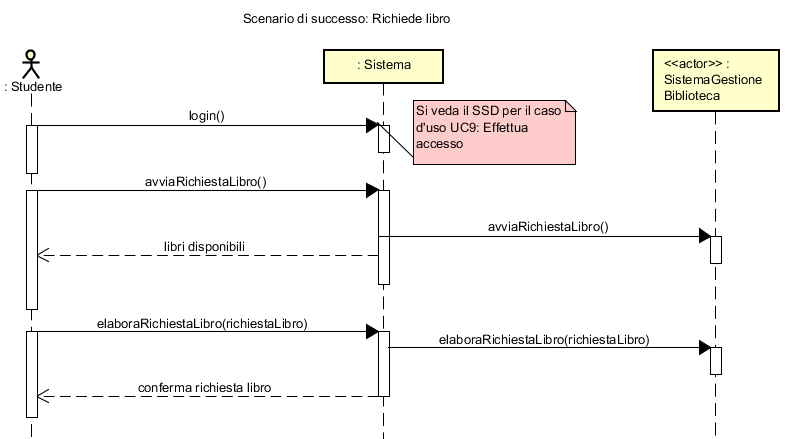
\includegraphics{./images/SSD_UC2.png}
	\end{center}

	\newpage

	\subsection{UC5: Gestisce corso}

	\begin{center}
		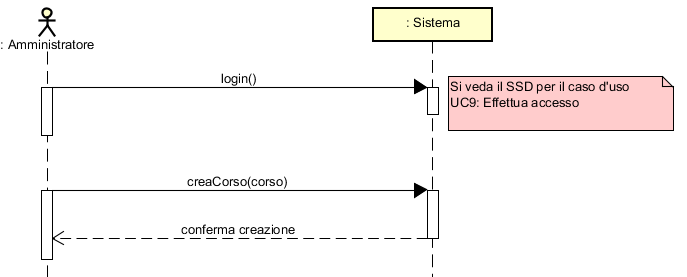
\includegraphics{./images/SSD_UC5.png}
	\end{center}

		%%%%%%% CONTRATTI
	
	\noindent\fbox{%
		\parbox{\textwidth}{%
			\large \textbf{Contratto CO1: creaCorso}\\
			
			\normalsize
			\textbf{Operazione:} \quad \quad creaCorso(corso)\\
			\textbf{Riferimenti:} \quad \quad Caso d'uso: Gestisce corso\\
			\textbf{Pre-condizioni:} \quad - Il Sistema è stato avviato.\\
			.\quad\quad\quad\quad\quad\quad\quad\quad\quad - L'Amministratore ha inserito il nuovo Corso\\ 
			\textbf{Post-condizioni:} \quad - Viene associata una voce del Registro Corsi\\
			.\quad\quad\quad\quad\quad\quad\quad\quad\quad al nuovo corso inserito
		}%
	}
	
	
	
	%%%%%%%%%%%% PROGETTAZIONE
	\newpage
	
	
	\section{Diagrammi di sequenza}
	
	I diagrammi di sequenza permettono di iniziare a progettare il software, partendo dall'analisi già effettuata. Essi mettono in evidenza le interazioni tra entità che sono già ottime candidate per diventari classi della programmazione orientata ad oggetti.
	
	A seguire si illustrano i diagrammi di sequenza relativi ai casi d'uso UC1 e UC5 che saranno implementanti durante questa Iterazione.
	
	\subsection{UC1: Indica tipo prenotazione}
	\begin{center}
		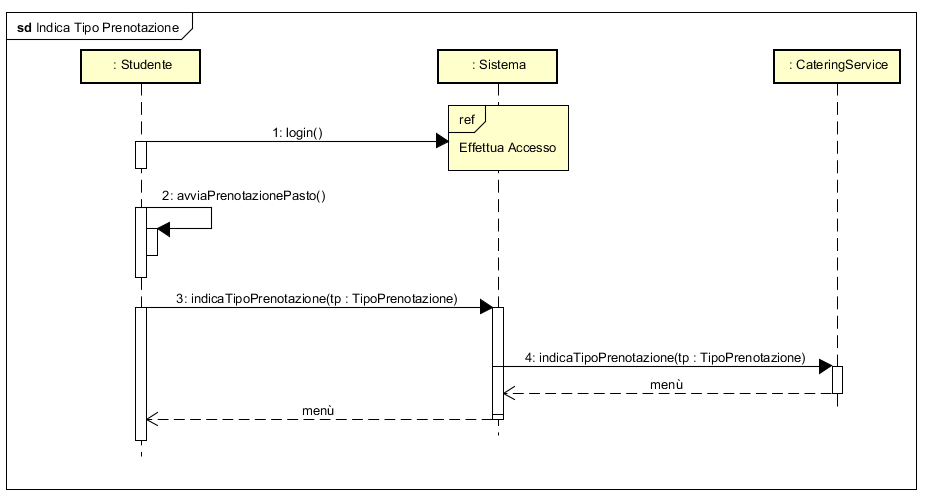
\includegraphics[scale=0.8]{./images/IndicaTipoPrenotazione.png}
	\end{center}

	\subsection{UC1: Elabora prenotazione}
	\begin{center}
		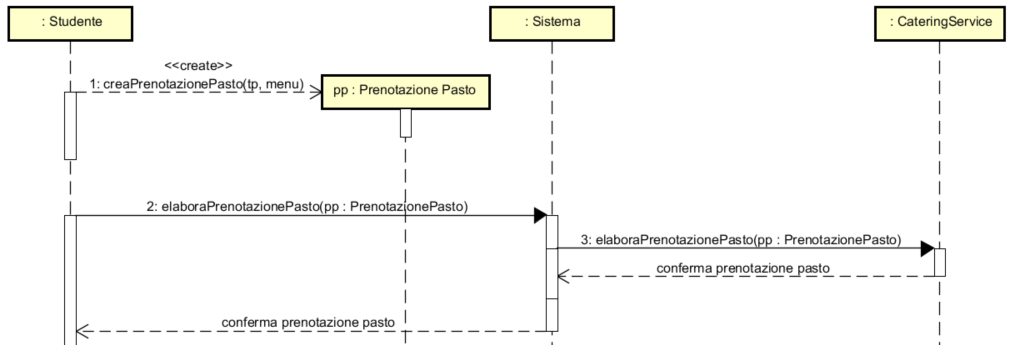
\includegraphics[scale=0.8]{./images/ElaboraPrenotazione.png}
	\end{center}
	
	\subsection{UC5: Aggiungi corso}
	\begin{center}
		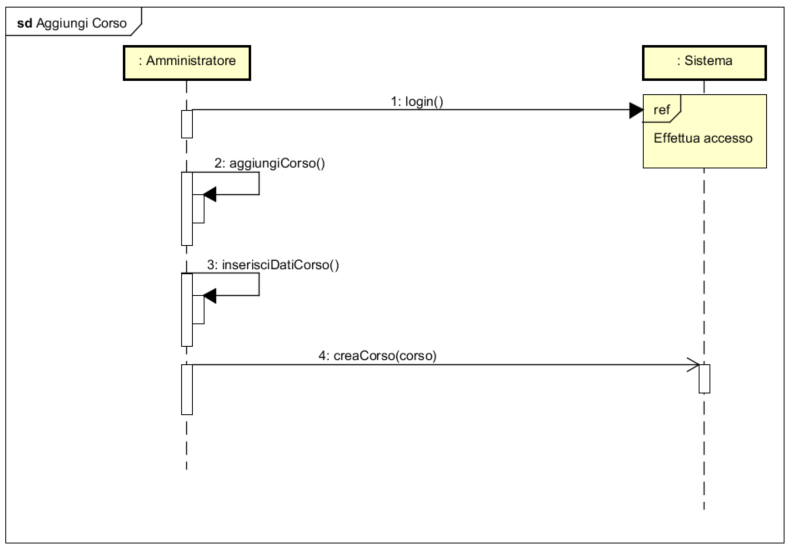
\includegraphics{./images/AggiungiCorso.png}
	\end{center}
		
	\subsection{UC8: Crea corso}
	\begin{center}
		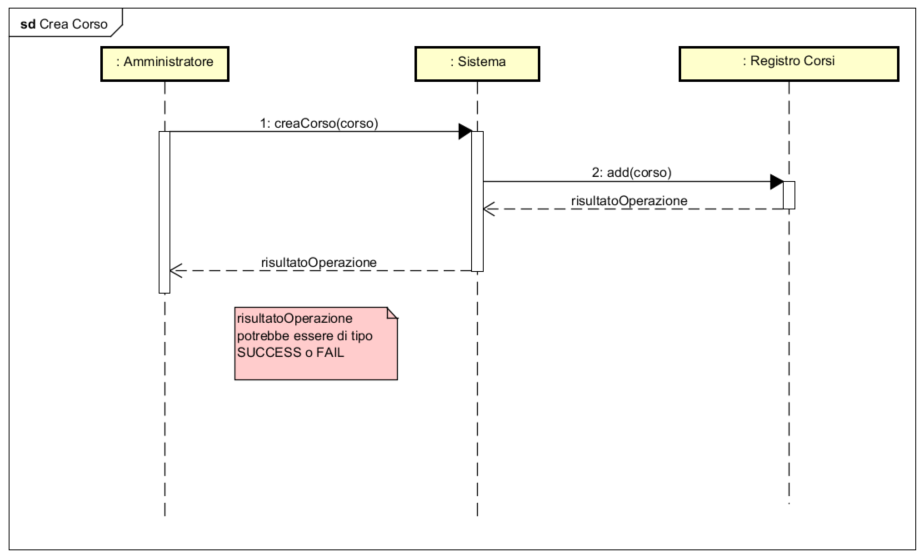
\includegraphics[scale=0.8]{./images/CreaCorso.png}
	\end{center}


	\newpage
	
	\section{Diagrammi delle classi e implementazione}
	
	Il Diagramma delle classi che segue è il risultato di un processo di raffinazione, ottenuto applicando pattern GRASP e alcuni Design Pattern [GOF], a partire dagli elaborati dell'analisi e della progettazione finora svolte.
	
	La sua stesura è avvenuta in maniera quasi parallela alla programmazione, per evidenziare fin da subito i punti critici e le difficoltà nella traduzione del diagramma in codice Java.	
	
	\begin{center}
				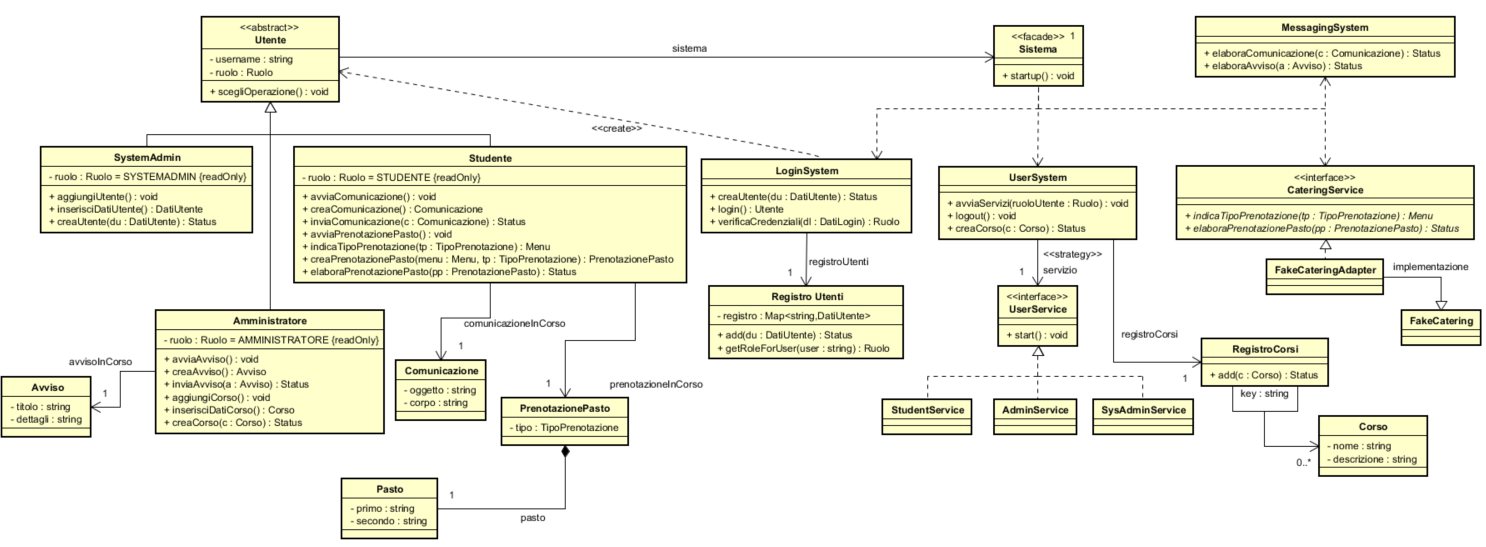
\includegraphics[scale= 0.6]{./images/DCD-I3.png}
	\end{center}

	Alla fine di questa iterazione sono stati implementati sei casi d'uso, di cui almeno 4 con alcune estensioni disponibili, oltre agli scenari di successo. Per quanto riguarda il caso d'uso \textit{UC1} andrebbero tenute in considerazione le regole di dominio (al momento solo una delle due è integrata nella piattaforma).
	
	L'integrazione di sistemi esterni, quale il servizio mensa,	ha permesso di applicare il design pattern [GOF] dell'Adapter, per la classe \textit{FakeCateringAdapter}, che rende il servizio di un \textit{FakeCatering} compatibile con l'interfaccia di Sistema \textit{CateringService}.
	
	Un simile approccio sarebbe stato applicato anche con il caso d'uso \textit{UC2: Richiede libro}.
	
	
	
	\newpage
	
	%%%%%%%%%%%% TESTING
	
	\section{Testing}
	
	Sono stati scritti oltre 20 test che verifichino il funzionamento dei metodi delle classi di sottosistema (quelle per cui \textit{System} fa da Facade).
	
	Per la suite di test a scatola nera sono stati scelti casi di uso normale (scenari di successo) e casi estremi, utilizzando input scelti in maniera specifica per il singolo test.
	
	Il resto del codice è stato testato manualmente cercando di coprire tutti i cammini percorribili.
	
	Con i test della suite JUnit si è raggiunta una copertura del 56\% del codice. Con i test manuali si è invece superato il 90\% di copertura.
	
	Nonostante ciò è possibile che il software celi ancora diversi errori, dovuti a valori di I/O errati (non ancora intercettati) o errori di riferimento ai dati. 
	
	
	
	
\end{document}